\section{Úvod do problematiky}
Saliency a teda detekcia významných oblastí je využívaná v rôznych oblastiach.
Automatizáciou sú modely významných oblastí (anglicky saliency modelov) ťažiskom pri segmentácii obrazu alebo detekcii špecifických objektov.
Od saliency modelov sú taktiež závislé aj programy ovládajúce zabezpečovacie zariadenia.
Tým, že zužujú možnosti a proaktívne upozorňujú na podozrivé situácie pomocou zúženia obrazu na zopár oblastí.
Saliency model používa aj oblasť reklamy, kde je vizuálna pozornosť kľúčovým parametrom, čo môže rozhodnúť o úspechu produktu.
Veď aký význam by mala reklama, kde si nevšimnete prezentovaný produkt alebo si všimnete iba jeho 'menej' dokonalé časti.
\section{Metódy pre statické obrazy}
Algoritmy pre statické obrazy tvoria základ všetkých saliency modelov a sú najstaršou oblasťou výskumu.
V tejto časti uvediem prehľad algoritmov pre výpočet saliency modelov od najjednoduchších cez najznámejšie až po najefektívnejšie.
Na záver uvediem porovnanie všetkých metód pomocou všeobecne uznávaných metrík a dát získaných zo zariadení merajúcich pohyb očí používateľa (eyetrackera).
\subsection{Baseline Center}\label{section:caseline-center}
Baseline center je triviálny model, ktorý sa vypočítava pomocou Gaussovej krivky vzhľadom na pomer strán, čím predpokladá salientné oblasti presne v strede obrazu.
Nezachytáva však žiadne sémantické aspekty videa, ako ani podvedomé informácie vnímanania obrazu, iba rozlíšenie dané optikou skenujúcou scénu.
\subsection{Hrany}
Skupinu algoritmov využívajúcu význačné prechody v obraze inak nazývame hrany.
Metódy tohoto typu sú vyžívané hlavne v prírodných scénach, kde nie je (sémanticky) význačný objekt.
Takéto metódy sa zakladajú priamo na štúdiu fyziologických vlastností ľudského vizuálneho systému.
Následná imitácia procesov odohrávajúcich sa na sietnici viedla ku vzniku saliency modelov generujúcich plausibilné výsledky\cite{edges-1}.
\subsection{Ittiho model}
Najznámejším modelom pre výpočet významných oblastí pre statické farebné obrazy je ittiho model navrhnutý v roku 1998.
Model zakladá na rozložení obrazu na tri základné charakteristiky obrazu a to na farbu, intenzitu a orientáciu.

\begin{figure}[H]
 \centering
 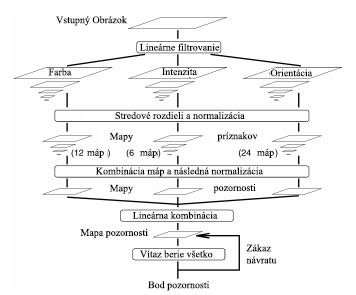
\includegraphics[width=7cm]{pics/itti-1-svk.png}
 \caption{Ucelená vizualizácia ittiho modelu\cite{itty-98}}\label{wrap-fig:1}
\end{figure}
\vspace{10mm}

Chrakteristika farby obsahuje 12 máp (šedotónové obrazy), pričom model používa farebný model RGB.
Na začiatku sa vypočíta intenzita podľa vzťahu \begin{math} I = (R+G+B)/3\end{math}.
Pomocou mapy I sa následne normalizujú všetky farebné kanály modelu RGB.
Model extrahuje štyri farebné kanály červený (r), zelený (g), modrý (b), žltý (y) a pomocou Gausvých pyramíd vytvorí tri rôzne mapy každej farebnej zložky separátne.
Červená zložka sa počíta difenčným spôsobom ako \begin{math} R = r - (g + b)/2 \end{math}, zelená ako \begin{math} G = g - (r + b)/2 \end{math}, modrá ako \begin{math}B = b - (r + g)/2\end{math} a žltá ako \begin{math}Y = (r + g)/2 - |r - g|/2 - b\end{math}.
Chrakteristika intenzity obsahuje šesť máp.
Získaná je pomocou orientovaných gáborových filtrov s orientáciou 0\degree, 45\degree, 90\degree, 135\degree.
Spolu 42 máp charakteristík je následne lineárne skombinovaných do jednej saliency mapy\cite{itty-98}.


\subsection{Spektrálne reziduá}
Metóda využíva princíp, že potláča štatisticky často opakujúce sa časti obrazu a do popredia stavia časti obrazu, ktoré sa štatisticky odlišujú od ostatných.
Na detekciu používa rýchlu fourierovu transformáciu.
Pomocou nej rozdelí obrázok na amplitúdovú časť a fázovú časť.

\begin{figure}[H]
  \centering
  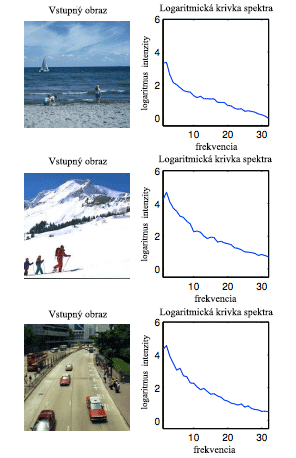
\includegraphics[width=10cm]{pics/spectral-img.png}
  \caption{Príklad rozloženia typovo rôznych obrazov\cite{spectral-rezidual}}\label{wrap-fig:2}
\end{figure}
\vspace{10mm}

Amplitúdová zložka sa následne vyhladí, čím sa do popredia dostanú iba informácie, ktoré sa vymykajú z priemeru.
Odčítaním od pôvodnej amplitúdovej zložky dostaneme iba časti obrazu, ktoré sú významné \cite{spectral-rezidual}.
\subsection{Sun Model}
Sun model (Saliency Using Natural statistics) sa snaží simulovať potencionálne ciele sledovania ľudského vizuálneho systému.
Model aktívne hodnotí tieto ciele odhadom pravdepodobnosti vzhľadom na všetky pozorované charakteristiky.
Charakteristiky sú spracovávané separátne a teda model nepočíta s chrakteristikami navzájom sa ovplyvňujúcimi.
Údaje získané zo všetkých charakteristík následne spracuje štatisticky.
Model zakladá hlavne na Bayesovom pravidle.
Ako výsledok hľadania potom udáva asymetrie v týchto štatistických štruktúrach\cite{sun-1}.
\subsection{Rare Model}
Výrazná väčšina modelov pozornosti typu bottom-up funguje ustáleným postupom, kde sa z pôvodného obrazu extrahuje definovaná množina chrakteristík paralelne a tie sa následne kombinujú alebo inak použijú na výpočet výslednej mapy pozornosti.
Rare model narvhuje sekvenčnú architektúru, kde z pôvodného obrázku extrahuje nízko úrovňové príznaky.
Následne na výsledkoch sériovo vykonáva extrakciu ďalších príznakov (v literatúre nazývané mid-level).
Nakoniec ako posledný krok spojí a normalizuje výsledné chrakteristiky do konečnej mapy významných oblastí.
Rare model ako nízkoúrovňové chrakteristiky používa jas a colorimetrické rozdiely (ako farebný model používa YCbCr) a následne na mapách rozložených zložiek farebného modelu detekuje orientáciu pomocou gáborových filtrov\cite{rare-1}.
Po extrakcii všetkých charakteristík použije iteratívnu metódu pre optimálne kvantovanie, založenú na metóde Otsu\cite{otsu}.
Na takto upravenom vstupe sa následne vyhľadávajú vzácne (z angl. rare) oblasti obrazu.
Metóda preskúmala možnosti nesekvenčnej extrakcie príznakov z obrazu, čo bolo novým prístupom v oblasti modelov pozornosti.

\begin{figure}[H]
  \centering
  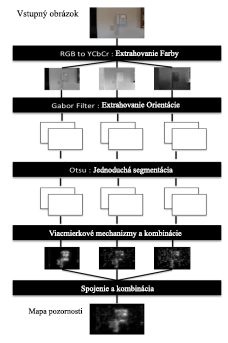
\includegraphics[width=6cm]{pics/rare-1-svk.png}
  \caption{Rare model workflow\cite{rare-1}}\label{wrap-fig:3}
\end{figure}

\section{Metódy pre videá}
Video obsahuje rozsiahlejšie možnosti ako obrazová informácia, pribúdajú ďalšie rozmery ako je pohyb objektov na obraze alebo vplyv zvuku na ľudské vnímanie.
Avšak oproti obrazu je potrebné spracovávať väčšie množstvo dát.
Navyše vo väčšine algoritmov využívajúcich saliency modely je potrebné, aby model dával výsledky v reálnom čase hlavne v oblasti zabezpečovacej techniky.
\subsection{Zohľadnenie audio informácie}
Saliency modely využívajú rôznorodé druhy príznakov a to od geneticky zakorenených, ako sú prechody farieb alebo intenzít, až po sémantické príznaky, ako je detekcia tváre \cite{salient-faces}.
Majoritná väčšina saliency modelov využíva iba obrazovú zložku, pričom zvuková stopa býva nevyužívaná alebo úplne zanedbaná.
Použitie zvuku je známym trikom filmovej scény už desatročia.
Režiséri posilňujú kontrolu nad diváckou pozornosťou práve pomocou zvukového doprovodu.
Prvé štúdie sa zaoberali detekciou reči a tváre, kde je spojitosť jednoznačná \cite{sound-1}.
Neskoršie štúdie dokazujú korelácie aj na všeobecnejšej úrovni a pokusy o extrakciu samotnej charakteristiky zo zvukovej stopy\cite{sound-coutrot-1}.
Tieto pokusy viedli aj k zostaveniu modelov zohľadňujúc zvukovú stopu ako samostatnú charakteristiku spolu s kombináciou nízkoúrovňových príznakov obrazu \cite{sound-courot-2}.

\begin{figure}[H]
  \centering
  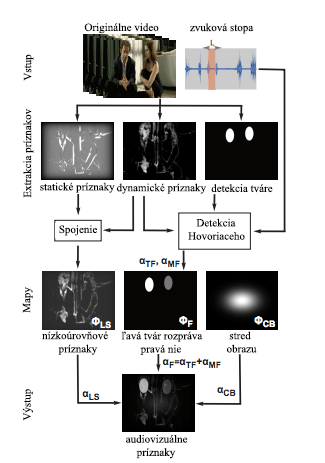
\includegraphics[width=9.5cm]{pics/courot-1.png}
  \caption{Vizualizácia audiovizuálneho modulu\cite{sound-courot-2}}\label{wrap-fig:4}
\end{figure}
\vspace{10mm}

Model extrahuje video na sekvenciu obrazov (framy) a audio stopu v tvare grafu vlnovej dĺžky.
Potom extrahuje tri typy rôznych chrakteristík.
Nízkoúrovňové príznaky založené na biologicky inšpirovaných saliency modeloch rozdelených na dynamickú časť a statickú časť.
Statická časť sa zameriava na najasnejšie a najkontrastnejšie časti obrazu.
Dynamická časť sa zameriava na relatívny pohyb objektov vhľadom na pozadie (eliminácia pohybu kamery).
Tieto dve časti sa nakoniec spoja.
Ďalšou chrakteritikou použitou v tomto modeli je detekcia tváre.
Každý objekt klasifikovaný ako tvár je v saliency mape nahradený oválnym objektom.
Intenzita daných objektov je daná pomocou metódy Speaker Diarization\cite{sound-courot-2}, ktorá detekuje podľa zvukovej stopy objekt, ktorý generuje zvuk.
Metóda predpokladá striedavú konverzáciu viacerých objektov oddelenú pauzou.
Následne spojí vyššie spomínané charakteristiky do jednej výslednej mapy.
Ako posledný krok preloží cez celú mapu baseline center model popísaný v časti \ref{section:caseline-center}.

\subsection{Detekcia pohybu}
Táto časť je zameraná na segmentáciu objektov, ktoré sa na scéne pohybujú.
Metódy tohoto typu sa snažia vizualizovať 3D prostredia (v našom prípade disponujeme výškou, šírkou a časom) na 2D výstup (obrazový výstup).
Takáto informácia dokáže priblížiť výpočtové modely bližšie k realite.
Ľudský vizuálny systém totiž nepoužíva iba 2d vstup (ako to prebieha v drvivej väčšine metód na výpočet významných oblastí).
Takéto obrazy sú v ľudskom vizuálnom systéme vysoko hodnotené.
Dôvody, prečo takto ľudský vizuálny systém zvyšuje prioritu práve takýmto oblastiam môžeme nájsť v antropológii.
Vysvetlenie je jednoduché a to snaha zabezpečiť bezpečné prostredie okolo seba a všetko pohybujúce sa narušuje pocit bezpečnosti.
V nasledujúcom texte rozoberieme dva najpožívanejšie algoritmy na detekciu oblastí pohybu v obraze a výpočet vektoru posunu.
Výpočet vektoru posunu je však iba projekcia 3D vstupných dát do 2D obrazu a nemusí vždy reprezentovať iba pohyb.
Prvým z nich bude LUCAS KANADE\cite{lucas-kanade} a druhým Horn Schunck\cite{horn-schunck}.
Obidva tieto algoritmy používajú jeden spoločný predpoklad a to, že jas daného objektu sa časom nemení.
To znamená, že objekt sa na scéne môže presunúť, ale svoj jas nemôže zmeniť.
Matematicky vyjadrené I(x(t),y(t),t) je obrazová dvojrozmerná funkcia, ktorá sa mení vzhľadom na čas.
Keďže sa jas obrazu nemení môžeme povedať, že platí:
\begin{equation}
  I(x + dx/dt \sigmat ,y + dy/dt \sigmat, t + \sigmat) = I(x,y,t)
\end{equation}
Z čoho je ľahko odvoditeľné, že:
\begin{equation}
  dI/dt = \sigmai/\sigmax dx/dt + \sigmai/\sigmay dy/dt + dI/dt  =  0
\end{equation}

\subsection{Lucas Kanande}
Algoritmus prvotne vznikol ako návrh pre časovú optimalizáciu problému výpočtu vektora posunu medzi dvomi krivkami.
Pôvodné primitívne riešenie vyžadovalo \begin{math} O(M^2 * N^2) \end{math} času pre výpočet daného vektora ak M,N bolo rozlíšenie daného obrazového vzoru.
Vtedy navrhovaná optimalizácia vyžadovala zadanie rozsahu hľadania, pomocou ktorého sa vypočítali diferencie pre celý obraz a pre ďalšiu iteráciu sa rozsah vypočítal pomocou horolezeckého algoritmu.
Metóda Lucas Kanade využíva priestorový gradient pre výpočet nových hodnôt a zároveň upravuje hodnotu rozsahu pri výpočte kažkého obrazového pixelu v obraze a nie iba po výpočte celého obrazu.
Pomocou takejto úpravy naivného algortimu sa časová zložitosť zlepšila na \begin{math} O(M^2 log N) \end{math}\cite{lucas-kanade}.

\begin{figure}[H]
  \centering
  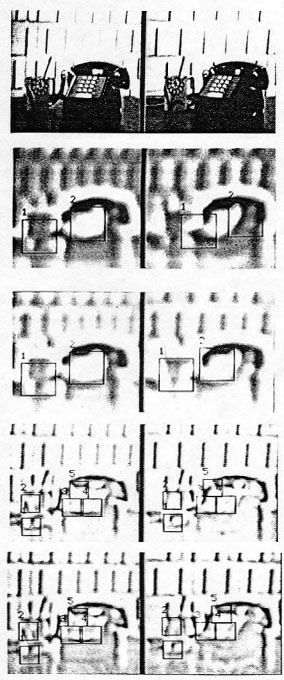
\includegraphics[width=7cm]{pics/lukas-kanade.jpg}
  \caption{Vizualizácie výsledkov algoritmu Lucas-Kanade vždy po 1 iterácii\cite{lucas-kanade}}
\end{figure}
\vspace{10mm}

\subsection{Horn-Schunck}
Metóda Horn-Schunck bola prvá, kde bola použitá metóda variácie na výpočet optického toku.
Táto globálna metóda priniesla výpočet  konštanty pre obmedzenie plynulosti optického toku.
Algoritmus používa dva základné parametre: počet iterácií a vyhladzovaciu konštantu.
Počet iterácií určuje dĺžku (počet cyklov) simulácie, vyhladzovacia konštanta je použitá po každom cykle simulácie kvôli zjemneniu prechodov a na výpočet optimálneho optického toku.

\begin{figure}[H]
  \centering
  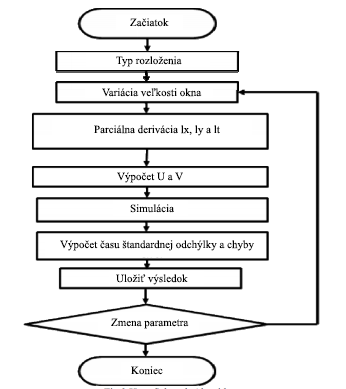
\includegraphics[width=7cm]{pics/horn-schunck.png}
  \caption{Vizualizácia pracovného postupu metódy Horn-Schunck}
\end{figure}
\vspace{10mm}

\section{Metriky úspešnosti}
Metriky úspešnosti sú algoritmy na čo najpresnejšie vyjadrenie presnosti modelov v meratelných jednotkách.
Takýto algoritmus dostáva na vstupe čisté dáta z eye trackera.
Tieto je potrebné predspracovať z dôvodu, že každý výrobca poskytuje iné zariadenia na hardwarovej úrovni a výrobcovia neštandardizujú výstup do jednotnej formy.
Následne je potrebné vytvoriť mapu fixácií, ktorá sa používa ako jeden zo vstupných parametrov v algoritmoch počítajúcich metriky úspešnosti.
\\
Metriky úspešnosti možno rozdeliť do troch štandardných skupín podľa druhu hodnôt, na ktoré porovnávajú reálne dáta (v literatúre nazývané ground truth) s vygenerovanými mapami význačných oblastí\cite{metrics-1}.
\begin{enumerate}
  \item\textbf{Založené na porovnávaní hodnôt} - NSS, Percentile, Pf
  \item\textbf{Založené na vyhodnocovaní vzdialeností} - AUC-Judd, AUC-Zhao, AUC Borji, AUC-Li
  \item\textbf{Založené na distribúcii} - KL-Div, EMD, CC, SRCC
\end{enumerate}

\subsection{NSS}
NSS (Normalized Scanpath Saliency) je metrika narvrhnutá v roku 2005, ktorej autormi sú R. J. Peters a L. Itti.
Metrika zakladá na ohodnotení salientných oblastí vzhľadom na pozíciu fixácií samostatne a následne hodnotu normalizuje vzhľadom na počet fixácií v celom obraze\cite{metrics-1}.
\\
Pre každú fixáciu používa vzťah
  \begin{equation}
    NSS(p) =  (SM(p)-\SI{}{\micro}_{SM}) / 	\sigma_{SM}
  \end{equation}
Kde SM je mapa význačných oblastí, p je bod danej fixácie, pre ktorú sa hodnota vypočítava.

Mapa fixácií SM je normalizovaná tak, aby nadobúdala nulovú strednú hodnotu a zároveň jednotkovú štandardnú dochýlku.
Metrika NSS nadhodnocuje, ak je na výslednej saliency mape minimálna rozmanitosť hodnôt (malý rozdiel medzi hodnotami fixácií a strednou hodnotou), pretože v takomto prípade nebude model dostatočne ohodnotený.
Ak hodnotený model nájde presné pozície a odchýlka je malá, alebo rozdiel medzi hodnotami fixácie a strednou hodnotou je vysoký.
Potom finálna hodnota NSS metriky je určená priemerom hodnôt pre všetky fixácie\cite{metrics-1}.

\begin{equation}
  NSS = 1/N * \sum_{p=1}^{N}NSS(p)
\end{equation}

\subsection{AUC-Judd}
Metrika je clasická AUC, ktorú navrhol Judd \cite{auc-judd}.
Ako prvé sa pixely označené ako fixácie spočítajú s rovnakým počtom náhodných pixelov vybraných z mapy význačných oblastí a nakoniec sú považované za klasifikátor úspešnosti.
Nasleduje prahovanie zvolenou hodnotou.
Pixely, ktoré sú menšie ako prahovacia hodnota sú pokladané za pozadie obrazu a pixely, ktoré majú hodnotu vyššiu sú pokladané ako fixácie.
Pre ľubovolne zvolenú prahovaciu hodnotu sú niektoré výsledné oblasti manuálne označené ako pozitívne (True Positives).
Pobobne niektoré oblasti, ktoré nie sú označené ako fixácie, sú manuálne označené ako falošne pozitívne (False Positive).
Tieto operácie sú zopakované tisíckrát, nakoniec sa vizualizuje pomocou ROC krivky a plocha pod krivkou (Area Under the Curve preto AUC) je výsledným klasifikátorom, ktorého ideálna hodnota je 1.
Hodnota náhodného výberu je 0.5.

\subsection{KL-Div}
KL-Div v literatúre nazývaná aj Kullback-Leiblerova divergencia\cite{kldiv} je bežne používaná aj mimo oblasti počítačového videnia, ako metóda pre odhad celkovej rozdielnosti medzi dvoma distribúciami.
Mnoho autorov saliency modelov používa túto metriku, ako hodnotu straty informácie tj. koľko informácií sa stratí po vypočítaní daného saliency modelu voči mape fixácií.
\\\\
Každý projekt vytvárajúci model významných oblastí si volí vlastné metriky úspešnosti, podľa ktorých sa určuje úspešnosť daného modelu.
Pre meranie úspešnosti modelov je okrem samotných algoritmov potrebné zabezpečiť dostatočne rôznorodú skupinu testovacích dát tzv. datasetov.

\section{Referenčné datasety}
Dataset je testovacia množina vstupov, ktorá sa snaží obsiahnuť dostatočne rôznorodé vzorky vhodné pre komplexné testovanie.
Pri zostavovaní datasetov sú dôležité nielen videá ale eyetracker data alebo nejakým spôsobom zverejnené fixácie (získané napríklad aj ručným označovaním významných oblastí), aby bolo možné výsledky validovať pomocou vyššie uvedených metrík.
Ďalšou charakteristikou datasetu je množsto ľudí na, ktorých boli dané viedeá nahrávané.
\\ Príklady datasetov:
\begin{itemize}
	\item \textbf{RSD}\cite{rsd}
	\item \textbf{SAVAM}\cite{savam}
	\item \textbf{Coutrot datasets}\cite{courot-dataset}
  \item \textbf{ASCMN}\cite{accv}
\end{itemize}

\subsection{RSD}
Regional Saliency Dataset sa snaží o čo najobšírnejšie testovanie a rôznorodosť videií.
Je rozdelený do 4 hlavných kategórií:
\begin{itemize}
	\item \textbf{bezpečnostné záznamy} - Štadardné záznamy z bezpečnostných kamier obsahujú statické pozadie a salientné pohybujúce sa objekty.
Pre túto časť datasetu boli využité záznamy z projektu CAVIAR\cite{rsd-caviar}.
	\item \textbf{Grafika} - Použité animované filmy/seriály ktoré obsahujú 2D aj 3D grafiku.
  \item \textbf{Prirodzené videá s prvkami grafiky} - Prirodzené videá  podobné bezpečnostným videám ale s prvkami umelo vloženými priamo do obrazového kanálu.
  \item \textbf{Prirodzené videá} - Videá bez pridaných grafických prvkov, tak ako boli nasnímané kamerou.
\end{itemize}

Na vyznačenie zaujímavých oblastí nebola zvolená technika (eyetracker) ale manuálne vyznačovanie zaujímavých oblastí pomocou používateľov.
Výskumu sa zúčastnilo 17 mužov 6 žien medzi 10-23 rokov veku, na označení každého z videa sa podielalo 10-23 ludí.

\begin{figure}[H]
 \centering
 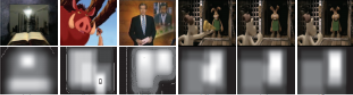
\includegraphics[width=7cm]{pics/rsd.png}
 \caption{Ukážka z každej kategórie videa s oznčenými významnými oblasťami}
\end{figure}
\vspace{10mm}

\subsection{SAVAM}
SAVAM (Semiautomatic Visual-Attention Modeling) je dataset nahrávaný priamo pomocou eyetrackera pri sledovaní videí v HD rozlíšení, pričom každému nahrávanému používateľovi sú pridelené dáta separátne pre kažké oko.
Spolu obsahuje 13 minút videa, ktoré bolo otestované na 50-tich používateľoch rôzneho veku.
Dataset je rozdelený na videá z filmov, ukážky z komerčných videí a na stereoskopické videá.
SAVAM taktiež poskytuje všetky raw dáta z eyetrackere ako aj vizualizácie daných dát\cite{savam}.

\subsection{ASCMN dataset}
ASCMN nazvaný podľa rozčlenenia do piatich skupín videa: abnormálne, bezpečnostné, videá s davom, videá s pohybom a videá s chybami v obraze (z anglických názvov: Abnormal, Surveillance, Crowd, Moving, Noise).
Spolu obsahuje 24 videí.
Každé video bolo namerané na 10-tich rôznych používateľoch.
K datasetu je taktiež dostupný validačný kód\cite{accv} počítavajúci hodnotiace metriky na ľubovolnom modeli pozornosti.

\subsection{Coutrot dataset}
Ide o dva rôzne datasety, obidva sú nazývané podľa authora Antoine Coutrota.
\textbf{Prvý dataset\cite{sound-1}} obsahuje videá s dynamickou povahou scény.
Je rozčlenený do štyroch vizuálne rozličných kategórií:
\begin{itemize}
  \item Jeden pohybujúci sa objekt
  \item Viacej pohybujúcich sa objektov
  \item Prírodné scény
  \item Konverzačné scény
\end{itemize}
Tento dataset obsahuje spolu 60 videí, ktoré sledovali vždy 18-tich rôznych používateľov.
Všetky videá boli zaznamenávané v štyroch rôznych zvukových podmienkach (využívať budeme iba dáta s pôvodnou zvukovou stopou). \\
\textbf{Druhý dataset \cite{coutrot-database-2}} obsahuje 15 videí.
Všetky videá obsahujú nahraté stretnutie štyroch konverzujúcich ľudí so statickou kamerou.
Dataset nie je členený do žiadnych kategórií.
Dáta oboch datasetov boli nahrávané pomocou eyetrackera EyeLink 1000 pri 1000Hz, pričom používatelia sedeli 57 cm od monitoru.
Eyetracker nahrával iba dáta z dominantného oka pre daného používateľa.

\section{Porovnanie štandardných metód}
Porovnávanie metód je štandardne publikované formou ucelených benchmarkov.
Príkladom takéhoto banchmarku je mit saliency benchmark\cite{mit-saliency-benchmark}, ktorý sa snaží zgrupovať a porovnávať obrazové modely pozornosti a zverejňovať referencie na ďalšie podobné projekty.
Na účely validácie bude vypracovaný podobný benchmark určený pre porovnanie rôznych modelov pozornosti na typovo rôznych datasetoch.
